\usetikzlibrary{patterns}
\usetikzlibrary{decorations.pathmorphing}
\usepackage{titlesec,calc}
% \renewcommand{\familydefault}{\sfdefault}

\titleformat{\section}[hang]
{\normalfont\bfseries}
{\thesection.}{0.5em}{}
 \titlespacing{\section}{0pt}{3pt}{0pt} % Horizontal space, before space, after space

\mode<presentation>
{
  \usetheme{CambridgeUS}
  \usecolortheme{whale}
  \usecolortheme{lily}

  \setbeamercovered{transparent}
  \usefonttheme[onlymath]{serif}
}

\title[Motor Control] % (optional, use only with long paper titles)
{\large \course: \coursename \\[5pt] \semesteryear\\[5pt] Exercise 2b: Motor Control}

\subtitle
{} % (optional)

\author[\instructorshort]% (optional, use only with lots of authors)
{\instructorlong\credits}
%{T. Vincent\inst{1} \and S.~Another\inst{2}}
% - Use the \inst{?} command only if the authors have different
%   affiliation.

\institute[\instituteshort] % (optional, but mostly needed)
{\institutelong}


\date % (optional)
{}



% If you have a file called "university-logo-filename.xxx", where xxx
% is a graphic format that can be processed by latex or pdflatex,
% resp., then you can add a logo as follows:

%\pgfdeclareimage[height=1.1cm]{university-logo}{UniversityLogo}
%\logo{\pgfuseimage{university-logo}}



% Delete this, if you do not want the table of contents to pop up at
% the beginning of each subsection:
%\AtBeginSection[]
%{
%  \begin{frame}<beamer>{Outline}
%    \tableofcontents[currentsection,currentsubsection]
%  \end{frame}
%}


% If you wish to uncover everything in a step-wise fashion, uncomment
% the following command:

%\beamerdefaultoverlayspecification{<+->}


\begin{document}



\begin{frame}
  \titlepage
\end{frame}

\mode<article>{
\maketitle
%\tableofcontents
}

%\mode<presentation>{
%\begin{frame}{Outline}
%  \tableofcontents
%  % You might wish to add the option [pausesections]
%\end{frame}}

\section{Introduction}
The purpose of this exercise is to design a control system that regulates the speed of a motor, and implement it using an Arduino. 

\section{The System}

A DC motor driving a wheel with bearing friction has the following ideal component representation.

\begin{center}
\begin{tikzpicture}[scale=1.75,inner sep=0pt,outer sep=0pt,very thick]
\draw (-1,-1) node (a) {}; 

\draw (-1,0) node (Va) {     \begin{tikzpicture}[scale=3] \useasboundingbox (-.11,.11) rectangle (.11,.89); 
    \draw[very thick] (0,.5) node[circle,draw,minimum width=.35in] (source) {\small$\begin{matrix} \mathbf{+} \\ \mathbf{-} \end{matrix}$};
    \draw[very thick] (0,.1) -- (source.-90);
    \draw[very thick] (source.90) -- (0,.9); 
    \end{tikzpicture}};
\draw (Va.180) node[left=6pt] {$v_{a}$};
\draw (0,1) node (R) { 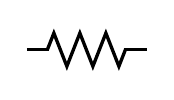
\begin{tikzpicture}[scale=1] 
 \useasboundingbox (-.25,-.28) rectangle (1.25,.28); 
 \draw[very thick] (-.26,0) -- (.02,0);
 \draw[very thick,decorate,decoration={zigzag,amplitude=6,segment length=9.4}] (0,0) -- (1,0);
 \draw[very thick] (1,0) -- (1.26,0); \end{tikzpicture}};
\draw (R.90) node[above=2pt] {$R_{a}$};
\draw (R) node[below=.15in] {$\begin{matrix} \longrightarrow \\ i_{a}\end{matrix}$};
\draw (1,1) node (L) {    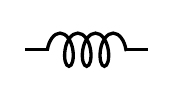
\begin{tikzpicture}[scale=1] \useasboundingbox (-.25,-.28) rectangle (1.25,0.28); 
    \draw[very thick] (-.28,0) -- (0.02,0);
    \draw[very thick,decorate,decoration={coil,segment length=6.4,amplitude=6}] (0,0) -- (1,0);
    \draw[very thick] (1,0) -- (1.28,0); \end{tikzpicture}};
\draw (L.90) node[above=2pt] {$L_{a}$};
\draw (2,0) node[circle,draw] (Vb) {\rule{0pt}{30pt}};
\draw (3.5,0) node (M1) {    \begin{tikzpicture}[scale=3] \useasboundingbox (.29,-.03) rectangle (.71,.04); 
    %\draw[very thick] (0,0) -- (.18,0);
    \draw[very thick] (.5,0) node[rotate=90,cylinder,draw,shape aspect=.2,inner sep=0pt] {\rule{.05in}{0in}\rule{0in}{.6in}};
    %\draw[very thick] (0.85,0) -- (1,0); 
    \end{tikzpicture}};
\draw (3.5,0) node {$J$} ++(0,-.6) node {\small wheel};
\draw[->] (M1.135) node[above] {$\theta$} ++(-.1,-.1) .. controls  ++(-.15,-.3) and ++(-.15,.3) ..  ++(0,-.8);
\draw[->] (M1.135) ++(-.3,0) node[above=2pt] {$\tau$} ++(-.1,-.1) .. controls  ++(-.15,-.3) and ++(-.15,.3) ..  ++(0,-.8);
\draw (5,0) node (K) {    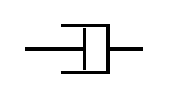
\begin{tikzpicture}[scale=3] \useasboundingbox (.26,-.09) rectangle (.74,.09); 
    \draw[very thick] (.25,0) -- (.5,0);
    \draw[very thick] (.5,-.09) -- (.5,.09);
    \draw[very thick] (.4,-.1) -- (.6,-.1) -- (.6,.1) -- (.4,.1);
    \draw[very thick] (0.6,0) -- (.75,0); \end{tikzpicture}};
\draw (K.90) node[above=4pt] {$b$};
\draw (6,0) node[rotate=180] (gnd) { 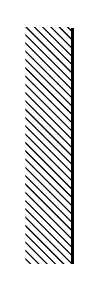
\begin{tikzpicture}[scale=3] \useasboundingbox (-.09,-.5) rectangle (.09,.5); 
    \fill[pattern=north west lines] (-.1,-.5) rectangle (.1,.5);
    \draw[very thick](.1,-.5) -- (.1,.5);
\end{tikzpicture}};


\draw (M1.0) -- (K.180);
\draw (K.0) -- (gnd.0);
\draw (2,0) -- (M1.180);
\draw (R.0) -- (L.180);
\draw (L.0) -| (Vb.90);
\draw (Va.90) |- (R.180);
\draw (Va) -- (a);
\draw (a.0) -| (Vb.-90);
\end{tikzpicture}
\end{center}

\section{Exercises}
\begin{itemize}
\item Mount the motor on a frame to make it stable, and add a wheel. Find the internal resistance and motor constants, using the specifications listed at \url{https://www.pololu.com/product/1444/specs}. 
You can assume $L_{a}=0$. For a specific value of $v_{a}$, use the stall torque and current and the relationship $\tau_{m}=K_{t}i_{a}$ to find $K_{t}$. With that same value of $v_{a}$, use the steady state circuit relationship $\frac{v_{a} - K_{e}\dot{\theta}}{R_{a}} = i_{a}$ with the free-run and stall values of $i_{a}$ and $\dot{\theta}$ (note that stall means $\dot{\theta}=0$) to give you two equations to solve for $K_{e}$ and $R_{a}$. Don't forget to convert to SI units. 
\begin{itemize}
\item If necessary, review Lecture 11, Motors and Hydraulic Actuators
\end{itemize}

\item Add a motor driver to the Arduino, hook up the motor driver to the motor with wheel attached, and use the Arduino to spin the motor, using the \texttt{analogWrite} command to command the motor driver to supply a pulse width modulated signal of a desired pulse width.  
\begin{itemize}
\item \url{https://www.pololu.com/product/1444}
\item \url{https://www.pololu.com/product/2503}
\end{itemize}
\item Use the Arduino to read the rotary encoder.
\begin{itemize}
\item \url{http://en.wikipedia.org/wiki/Rotary_encoder#Incremental_rotary_encoder}
\item \url{http://playground.arduino.cc/Main/RotaryEncoders} (Use the high performance encoder library)
\end{itemize}
\item Set up an Arduino program that will perform a step response experiment. This program should have a main() function that runs at a fixed cycle time, also called the sampling time. Use the function \textsf{micros} or \textsf{millis} to control the sample rate, by waiting at the end of your main function until the correct time has passed since the last time through. Have the program read the angular position, and from this data and the known sampling rate, calculate the angular velocity. For the step experiment, the program will initially output a motor voltage command of 0, changing to a desired positive value at 1 second. (By motor voltage command, we mean the value used in the \texttt{analogWrite} function; this should be a number between 0 and 255.) Use the serial link to output the results. Use a sampling rate of about 1ms.
\item Perform a step response experiment, and estimate the transfer function from motor voltage command to angular velocity. Although the motor is theoretically second order, when the motor inductance is small, the response can be well approximated as first order. You will probably use a voltage command greater than 1, so don't forget to scale the results appropriately. 

\begin{itemize}
\item 307 Notes: Lecture 15, System Identification
\end{itemize}

\item Create a simulation that replicates your step response experiment. By attaching the wheel, you have added a load which can be model by an inertia and damper, which has transfer function $\frac{\dot{\theta}(s)}{\tau(s)}=\frac{1}{Js+b}$, where $J$ and $b$ are parameters that you will have to find. The motor block diagram is of the form
\begin{center}\resizebox{5in}{!}{
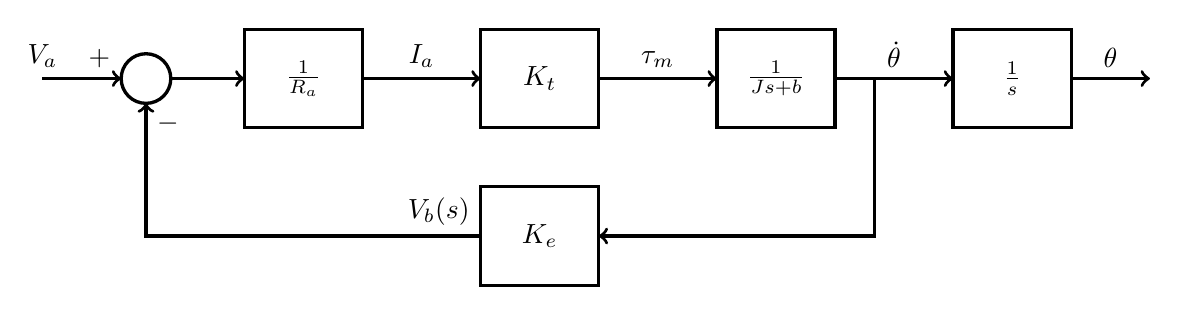
\begin{tikzpicture}[inner sep=0pt,outer sep=0pt,very thick,
sysblock/.style={draw,rectangle,inner sep=2pt,minimum width=1.5cm,minimum height=1.25cm,very thick}]

\draw (0,0) node[draw,circle] (sum) {$\rule{0pt}{18pt}$};
\draw (2,0) node[sysblock] (a) {$\frac{1}{R_{a}}$};
\draw (5,0) node[sysblock] (b) {$K_{t}$};
\draw (8,0) node[sysblock] (e) {$\frac{1}{Js+b}$};
\draw (11,0) node[sysblock] (c) {$\frac{1}{s}$};
\draw (5,-2) node[sysblock] (d) {$K_{e}$};

\draw[<-] (sum.180) node[above left=4pt] {$+$} -- ++(-1,0) node[above=4pt] {$V_{a}$};
\draw[->] (sum.0) -- (a.180);
\draw[->] (a.0) -- node[above=4pt] {$I_{a}$} (b.180);
\draw[->] (b.0) -- node[above=4pt] {$\tau_{m}$} (e.180);
\draw[->] (e.0) -- node[above=4pt] {$\dot{\theta}$} (c.180);
\draw[->] (c.0) -- node[above=4pt] {$\theta$} ++(1,0) ;
\draw[->] (e.0) -- ++(.5,0) |- (d.0);
\draw[->] (d.180) node[above left=4pt] {$V_{b}(s)$} -| (sum.-90) node[below right=4pt] {$-$};
\end{tikzpicture}}
\end{center}
From above, find the transfer function $\frac{\dot{\theta}(s)}{V_{a}(s)}$, and choose $J$ and $b$ so that the step response of this transfer function matches the one you found in the experiment. In your simulation, add blocks that account for non-ideal effects such as the discrete nature of the encoder. For example, since the motor position is read using the encoder, the position is quantized to one of 3200 counts per revolution. We can simulate this using quantization block (in \textsf{Discontinuities} folder, or search for quantizer) with a quantization interval of \texttt{2*pi/3200}. The position is only read periodically, so we need to simulate the sampling process. This is done by using a \textsf{Zero-Order-Hold} block (found in the \textsf{Discrete} folder), with the sampling time set to the sampling rate of your Arduino program. Finally, you can implement the code that you use to calculate the velocity from the measured position using either a Matlab function block or a \textsf{Discrete-Derivative} block. The resulting simulink block diagram will look something like the following:
\begin{center}
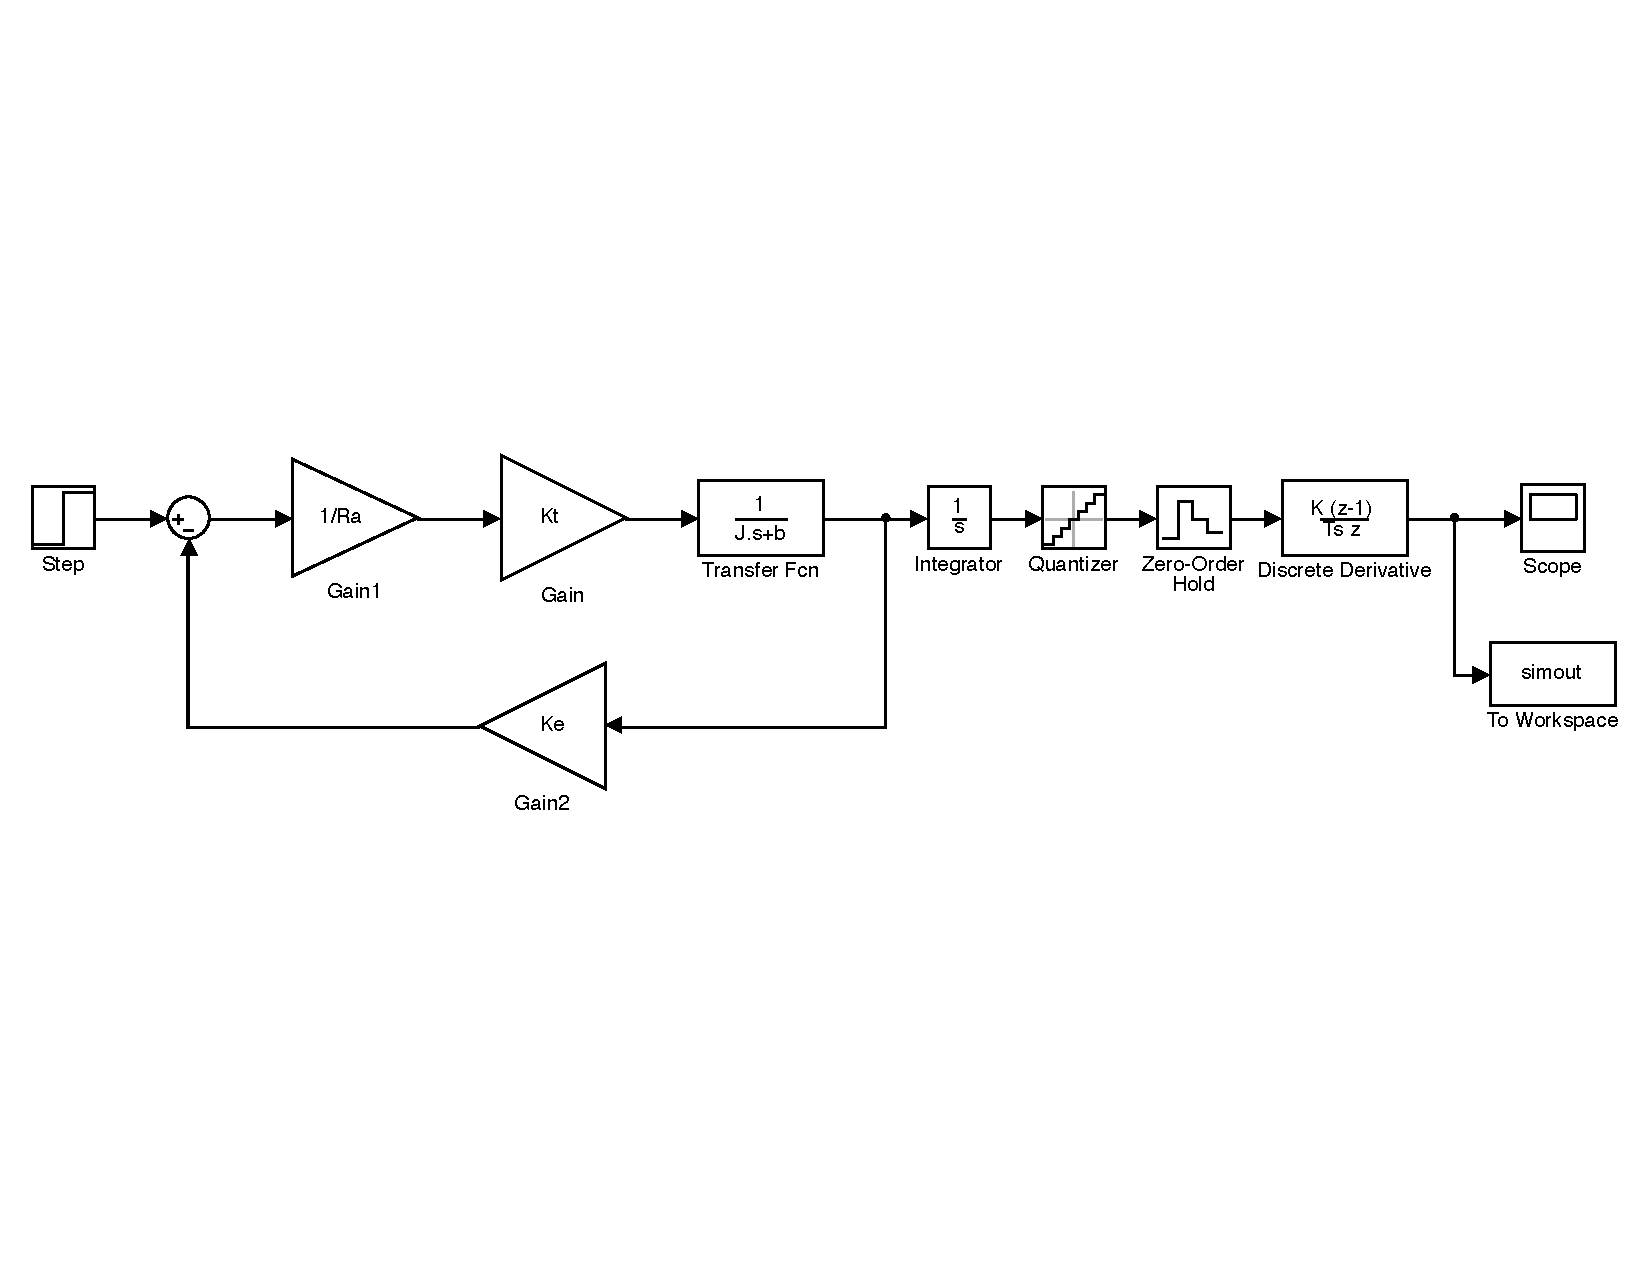
\includegraphics[width=6in]{figures/motor_simulation}
\end{center}
\item Using the transfer function $\frac{\dot{\theta}(s)}{V_{a}(s)}$ as the system to be controlled, design a PI controller to regulate the motor speed. That is, you should be able to specify a desired rotational velocity that the wheel will turn, even if there are disturbances. Aim for specifications of a rise time of 150 ms and an overshoot of less than 5\%.  Document your design procedure. (You can check your design against the autotune function of the Simulink PID block, but you should not use this as your primary design mechanism.) Simulate the closed loop system in Simulink.
\begin{itemize}
\item 307 Notes: Lecture 19, PID Control
\end{itemize} 
\item Implement the controller using the Arduino. Don't forget about units! 
\begin{itemize}
\item 307 Notes: Lecture 19, PID Control, Appendix.
\end{itemize}
Find the closed loop step response (that is, going from a setpoint of 0 to a setpoint of 1 rad/s), and compare to what you predicted from your design.







\end{itemize}





\section{Reporting}
\begin{itemize}
\item Document results, such as 
\begin{itemize}
\item your control design and design method
\item the simulated motor response, and 
\item the actual motor response. 
\end{itemize}
\item Document and store simulink and arduino code you can use to verify the motor controller is working correctly. That is, you should be able to quickly simulate a step response, and perform an experimental step response, and quickly compare the results in Matlab.
\end{itemize}
\section{Appendix 1: Verifying a Discrete Time Controller Using Simulink}

An easy way to simulate your embedded processor in Simulink, is to use a Matlab function block.  The Matlab function block can be found in the User-Defined Function library. If you drag it into your Simulink block diagram, and double click on the function, it will open the Matlab editor. The following code can be used to implement a PI controller using the Matlab function block. Variables that need to be remembered between function called are defined as \texttt{persistent}.
\begin{alltt}
function u = fcn(e,t)
\%\% Define Variables
\% Control Gains
Kp=1;
Ki=1;
umax = 10;
\% Memory variables
persistent I_past;
persistent t_past;
if isempty(I_past), I_past=0; end;
if isempty(t_past), t_past=0; end;

\%\% Calculate Controller
Ts = t - t_past;
\% Integrator
I = I_past+e*Ts;
\% PI control calculation
u = Kp*e+Ki*I;
if abs(u)>umax,
\rule{0pt}{0pt}\hspace{.1in}u = sign(u)*umax;
\rule{0pt}{0pt}\hspace{.1in}I = (u-Kp*e)/Ki;
end;
I_past=I;
t_past=t;
\end{alltt}

The following block diagram shows a Simulink block diagram with one loop implemented using a PI controller, and another implemented using the Simulink block. The zero order hold block is used to choose the sample rate. This can be entered by double clicking on the element. We have also added a clock so the Matlab function knows the elapsed time.

\begin{center}
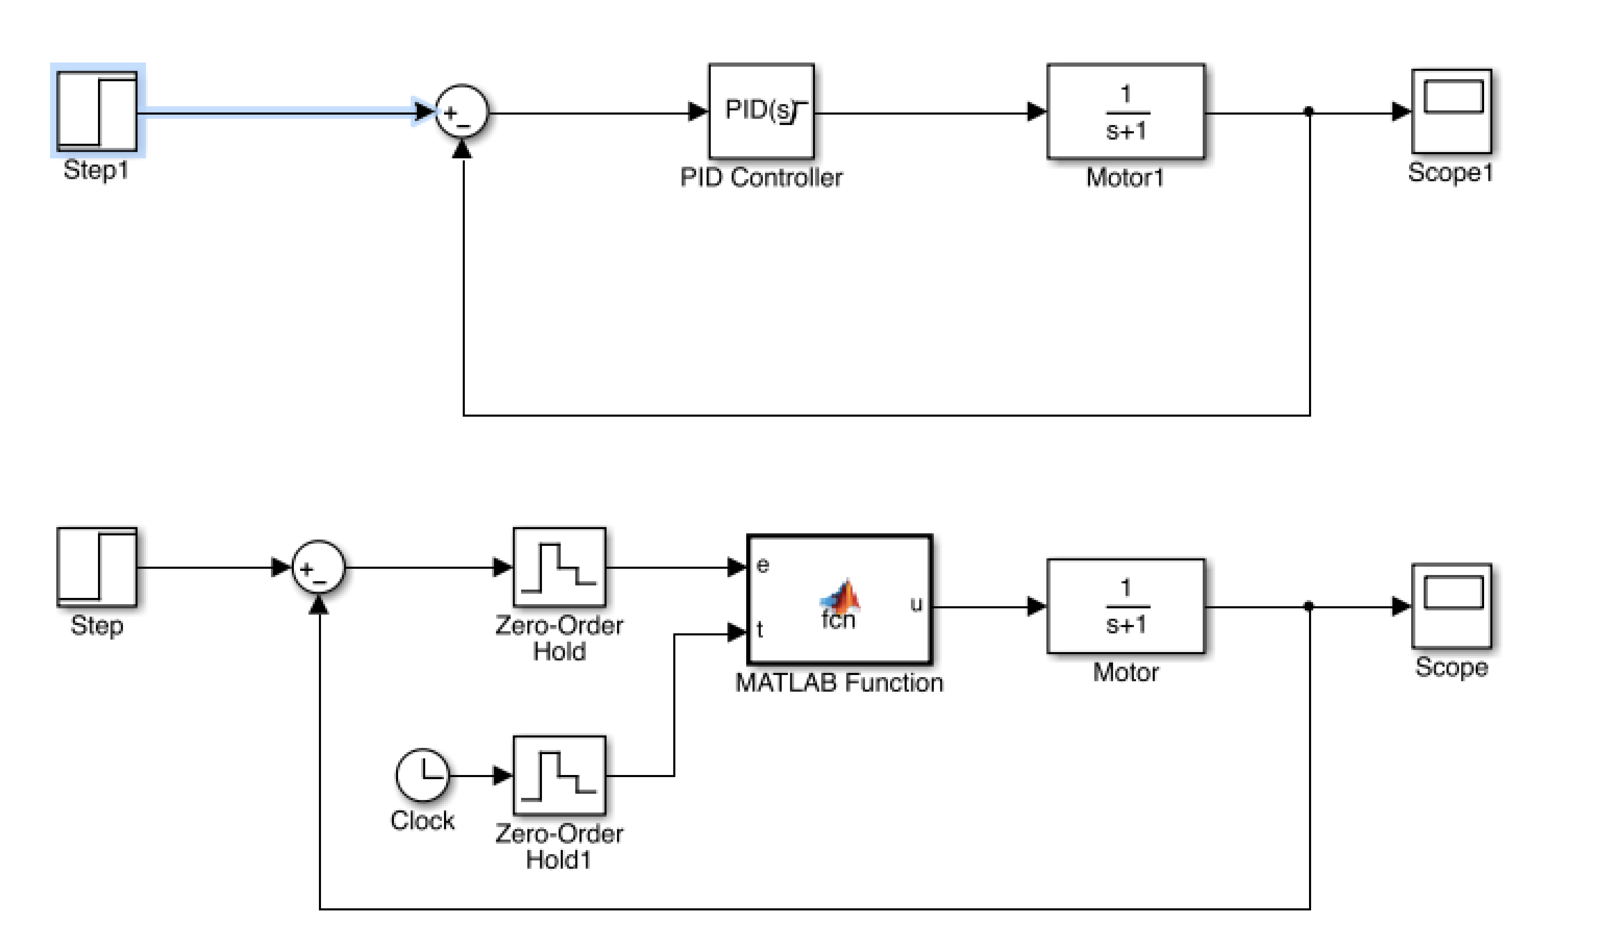
\includegraphics[width=5in]{figures/control_implementation}

\end{center}

%\section{Appendix 2: Simulation of a Robot}
%
%When your team starts designing their robot, you will want to be able to simulate how that robot will move in response to the motor. You will not need to do this for the preliminary demos, but the following describes how to integrate the motor and robot models.
%
%Create a copy of the Simulink block diagram you made for the robot and add components so that $u$ is a force applied by the motor. You can do this by creating a subsystem for the robot that has $f$ as the input and the important signals as outputs (see below). Creating subsystems was covered in the Simulink tutorial video. Integration of the motor block diagram with the robot simulation will then look like the following:
%
%\begin{center}\resizebox{5in}{!}{
%\begin{tikzpicture}[inner sep=0pt,outer sep=0pt,very thick,
%sysblock/.style={draw,rectangle,inner sep=2pt,minimum width=1.5cm,minimum height=1.25cm,very thick}]
%
%\draw (0,0) node[draw,circle] (sum) {$\rule{0pt}{18pt}$};
%\draw (2,0) node[sysblock] (a) {$\frac{1}{R_{a} + L_{a}s}$};
%\draw (5,0) node[sysblock] (b) {$K_{t}$};
%\draw (8,0) node[sysblock] (c) {$\frac{1}{r}$};
%\draw (11,0) node[sysblock] (e) {\textsf{Robot}};
%\draw (5,-2) node[sysblock] (d) {$K_{e}$};
%\draw (8,-2) node[sysblock] (f) {$\frac{1}{r}$};
%
%\draw[<-] (sum.180) node[above left=4pt] {$+$} -- ++(-1,0) node[above=4pt] {$V_{a}(s)$};
%\draw[->] (sum.0) -- (a.180);
%\draw[->] (a.0) -- node[pos=.5,above=4pt] {$I_{a}(s)$} (b.180);
%\draw[->] (b.0) -- node[pos=.5,above=4pt] {$\tau_{m}(s)$} (c.180);
%\draw[->] (e.0) -- ++(1,0) node[right=4pt] {$\dot{\phi}(s)$};
%\draw[->] (e.30) -- ++(1,0) node[right=4pt] {$X(s)$};
%\draw[->] (e.-30) -- ++(1,0) node[right=4pt] {$\dot{X}(s)$};
%\draw[->] (e.-30) -- ++(.5,0) |- (f.0);
%\draw[->] (f.180) -- node[above=4pt] {$\dot{\theta}(s)$} (d.0);
%\draw[->] (c.0) -- node[above=4pt] {$F(s)$} (e.180);
%\draw[->] (d.180) node[above left=4pt] {$V_{b}(s)$} -| (sum.-90) node[below right=4pt] {$-$};
%\end{tikzpicture}}
%\end{center}
%Note that the torque output from the motor divided by the wheel radius $r$ is the force applied to the robot, and the angular velocity of the motor shaft is the horizontal velocity divided by the wheel radius. It will be useful to animate the results of this simulation using the animation program you created in the previous exercise.


\end{document}


